\documentclass[11pt]{article}
\usepackage[toc,page]{appendix}
\usepackage{amsmath, amssymb}
\usepackage[utf8]{inputenc}
\usepackage[T1]{fontenc}
\usepackage[style=apa,backend=biber]{biblatex}
%\usepackage{biblatex}
\addbibresource{references.bib}
\usepackage{graphicx}
\usepackage{tikz}
\usetikzlibrary{automata,positioning,shapes.geometric, arrows.meta, fit, backgrounds, calc, chains}
\graphicspath{./images/Easy_Pictures/SMR_MULT_Repackaging}%\usepackage{kpfonts}
\usepackage{float}
\usepackage[margin=1in]{geometry}
\usepackage{cancel}
\usepackage{epsfig}
\usepackage{tikz-3dplot}
\usepackage{darkmode}
\usepackage{dirtytalk}
\usepackage{longtable,booktabs,array}
\usepackage{calc} % for calculating minipage widths
\usepackage[utf8]{inputenc}
\usepackage[T1]{fontenc}
\usepackage{xcolor}
\usepackage{listings}


\usepackage{etoolbox}
\usepackage{hyperref}
\hypersetup{
    colorlinks=true,
    linkcolor=blue,
    filecolor=magenta,      
    urlcolor=cyan,
    pdftitle={Hermeneutic Calculator},
    citecolor=blue,
    }


\urlstyle{same}

\lstdefinestyle{htmlStyle}{
    language=HTML,
    basicstyle=\ttfamily\small,
    keywordstyle=\color{blue}\bfseries,
    commentstyle=\color{gray}\itshape,
    stringstyle=\color{red},
    breaklines=true,
    frame=single,
    numbers=left,
    numberstyle=\tiny\color{gray},
    columns=fullflexible,
}
\lstdefinelanguage{HTML}{
  keywords={<!DOCTYPE, html, head, title, body, h1, h2, h3, p, div, span, a, img, ul, li, table, tr, td, th, style, link, script},
  sensitive=true,
  comment=[l]{//},
  morecomment=[s]{/*}{*/},
  morestring=[b]',
  morestring=[b]"
}
\lstset{style=htmlstyle, language=html}
% Updated to explicitly pass the language option
%\lstinputlisting[style=htmlstyle, language=html]{./html/example.html}
%\usepackage{tocloft}

% Optional: define some custom colors
\definecolor{sliceRed}{RGB}{225,224,91} % matching "varyellow" from your code
\definecolor{linkYellow}{RGB}{255,215,0}  % a golden yellow
\tdplotsetmaincoords{70}{110}

\title{Subtraction Strategies: Rounding and Adjusting}
\author{Theodore M. Savich}


\title{Multiplication Strategies: Commutative Reasoning}
\author{Compiled by: Theodore M. Savich}


\begin{document}
\maketitle
\subsection*{Commutative Action for Multiplication}

Imagine a situation where we have six chocolate chip cookies with 4 chocolate chips in each cookie. That's 24 chocolate chips. Instead, we imagine we have four chocolate chip cookies, and each cookie has 6 chocolate chips. That's still 24 chocolate chips, but not enough cookies to feed 4 kids! The commutative property of multiplication,
\begin{itemize}
    \item \textbf{Definition:} For any two natural numbers \( a \) and \( b \), 
    \[
    a \times b = b \times a.
    \]
    \item \textbf{Example:} \( 3 \times 4 = 4 \times 3 \).
\end{itemize}
is fine for purely abstract mathematical contexts, but in \textit{equal groups multiplication problems} -- the sort of problems that most people encounter when learning about multiplication for the first time -- the order of the factors can make a big difference.

However, there is a big difference between recognizing the commutative property holds for the number of chocolate chips and the fact that you would have two crying kids if there were 6 kids and you only had 4 cookies. 


For equal groups multiplication: 

\begin{equation*}
    \fbox{\text{number of groups}} \times \fbox{\text{number of items in each group}} = \fbox{\text{total number of items}}
\end{equation*}

To act (or reason) commutatively, the number of items in a group needs to be repackaged as the number of groups, while the number of groups transforms into the number of items in each group.


\subsubsection*{Definition and Example}
Imagine this situation, from \textcite{HackenbergCourseNotes}: we have ten packages of rainbow flavored candies, and each package contains the 7 candies, one of each of the `colors of the rainbow': red, orange, yellow, green, blue, indigo, and violet. 

It can be hard to count 7 objects ten times. $7+7+7+7+7+7+7+7+7+7$ is a lot of work! We can \textit{repackage} the candies into seven packages of 10 candies each - all the reds together, all the oranges together, and so on. The result is seven 10s, which is a lot easier to count: $10+10+10+10+10+10+10=70$. 

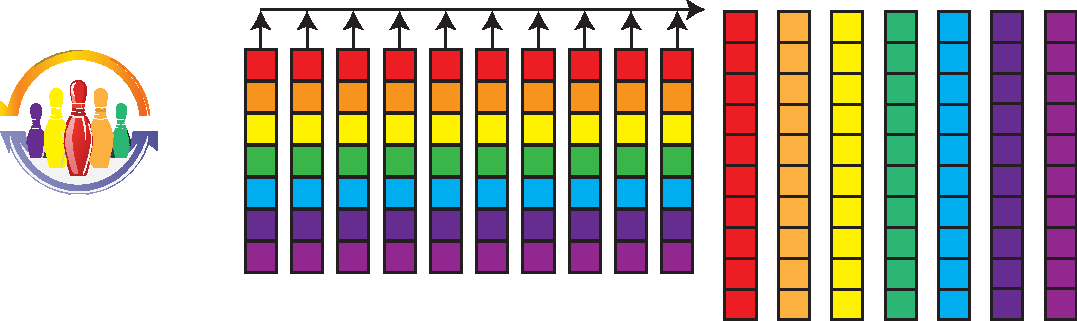
\includegraphics[width=.9\textwidth]{./images/Easy_Pictures/SMR_MULT_Repackaging/PDF/SMR_MULT_Repackaging.pdf}
\subsection*{Objective of the Automaton}
\begin{itemize}
    \item \textbf{Input:} A multiplication expression \( a \times b \).
    \item \textbf{Output:} The transformed expression \( b \times a \).
    \item \textbf{Functionality:} Recognize when a multiplication expression is presented and apply the commutative property to reorder the operands.
\end{itemize}

\subsection*{Automaton Type Selection}

\subsubsection*{Finite State Transducer (FST)}
\begin{itemize}
    \item \textbf{Transduction Capability:} Unlike finite state automata (FSA) that merely recognize languages, an FST can transform input strings into output strings.
    \item \textbf{Suitability:} Ideal for tasks involving input-output transformations, such as repackaging operands in a multiplication expression.
\end{itemize}

\subsection*{Designing the FST for Commutative Reasoning}

\subsubsection*{Components of the FST}
\begin{enumerate}
    \item \textbf{States (\( Q \))}:
    \begin{itemize}
        \item \( q_0 \): Start state.
        \item \( q_1 \): Reading the first operand.
        \item \( q_2 \): Reading the multiplication symbol (\( \times \)).
        \item \( q_3 \): Reading the second operand.
        \item \( q_4 \): Applying the commutative transformation.
        \item \( q_{\text{accept}} \): Accepting state; transformation complete.
    \end{itemize}
    \item \textbf{Input Alphabet (\( \Sigma \))}:
    \begin{itemize}
        \item Digits: \( \{0,1,2,3,4,5,6,7,8,9\} \)
        \item Multiplication symbol: \( \times \)
    \end{itemize}
    \item \textbf{Output Alphabet (\( \Delta \))}:
    \begin{itemize}
        \item Digits: \( \{0,1,2,3,4,5,6,7,8,9\} \)
        \item Multiplication symbol: \( \times \)
    \end{itemize}
    \item \textbf{Transition Function (\( \delta \))}:  
    Defines how the FST transitions between states based on input symbols and produces corresponding output symbols.
    \item \textbf{Start State:} \( q_0 \)
    \item \textbf{Accepting State:} \( q_{\text{accept}} \)
\end{enumerate}

\subsubsection*{Transition Function Details (Single-Digit Operands)}
For simplicity, assume operands are single digits. The FST behaves as follows:
\begin{center}
\begin{tabular}{|c|c|c|c|c|}
    \hline
    \textbf{Current State} & \textbf{Input Symbol} & \textbf{Read Symbol} & \textbf{Next State} & \textbf{Output Symbol} \\
    \hline
    \(q_0\) & Any digit \(d_1\) & \(d_1\) & \(q_1\) & \(d_1\) \\
    \(q_1\) & \( \times \) & \( \times \) & \(q_2\) & \( \times \) \\
    \(q_2\) & Any digit \(d_2\) & \(d_2\) & \(q_3\) & \(d_2\) \\
    \(q_3\) & End of input & --- & \(q_4\) & --- \\
    \(q_4\) & --- & --- & \(q_{\text{accept}}\) & Output repackaged \\ 
    & & & & expression: \(d_2 \times d_1\) \\
    \hline
\end{tabular}
\end{center}

\subsection*{Automaton Diagrams}

\subsubsection*{Circular Diagram for Single-Digit Operands}
Below is the circular state diagram for the FST (with the start and accept states merged) for single-digit operands.

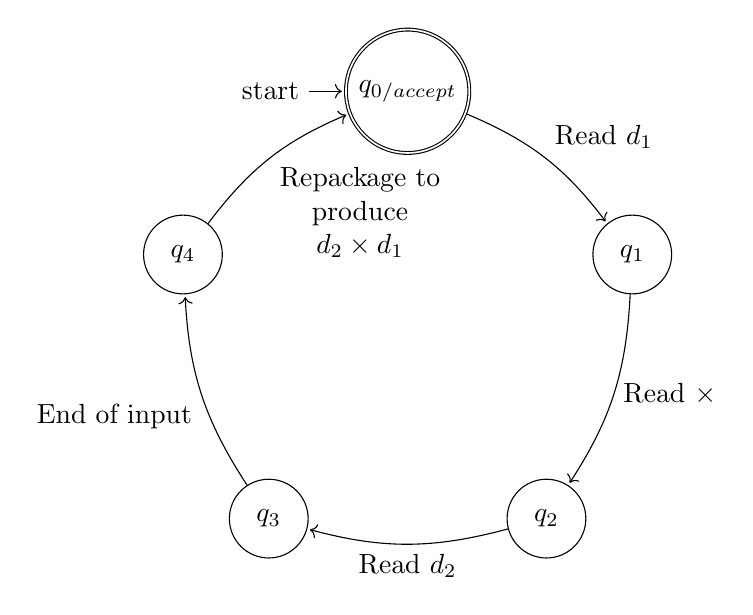
\begin{tikzpicture}[
    shorten >=1pt,
    auto,
    node distance=3cm,
    every state/.style={minimum size=1cm}
]
    % Arrange 5 states on a circle:
    \node[state, initial, accepting] (q0) at (90:3cm) {$q_{0/accept}$};
    \node[state] (q1) at (18:3cm) {$q_1$};
    \node[state] (q2) at (-54:3cm) {$q_2$};
    \node[state] (q3) at (-126:3cm) {$q_3$};
    \node[state] (q4) at (-198:3cm) {$q_4$};

    \path[->]
        (q0) edge[bend left=15] node[above right, align=center] {Read \(d_1\)} (q1)
        (q1) edge[bend left=15] node[right, align=center] {Read \( \times \)} (q2)
        (q2) edge[bend left=15] node[below, align=center] {Read \(d_2\)} (q3)
        (q3) edge[bend left=15] node[below left, align=center] {End of input} (q4)
        (q4) edge[bend left=15] node[below right, align=center] {Repackage to\\ produce\\ \(d_2 \times d_1\)} (q0);
\end{tikzpicture}

\subsubsection*{Circular Diagram for Multi-Digit Operands}
For multi-digit operands, the FST buffers digits until the entire operand is read, then repackages the operands. The following circular diagram represents an enhanced FST:

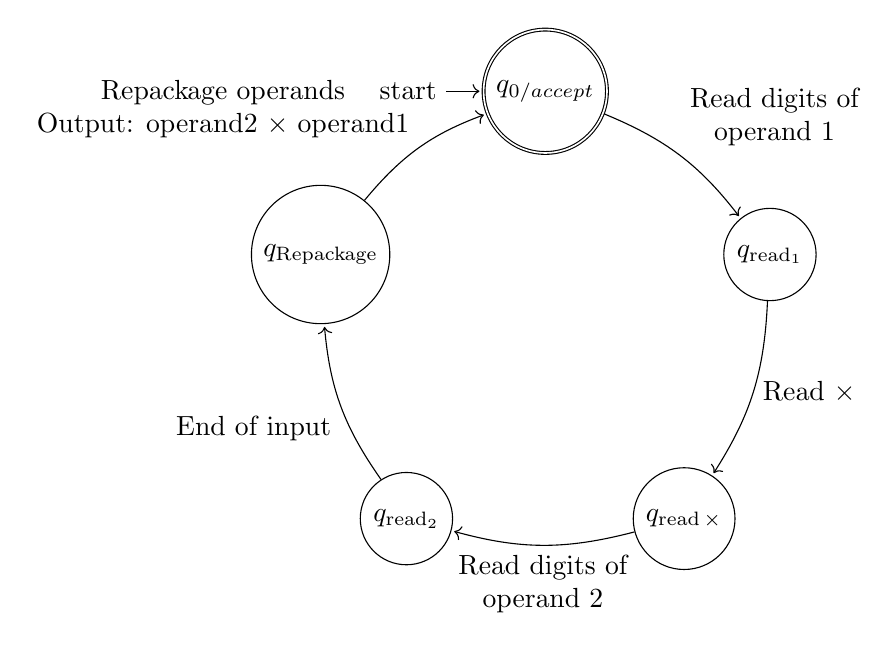
\begin{tikzpicture}[
    shorten >=1pt,
    auto,
    node distance=3cm,
    every state/.style={minimum size=1cm}
]
    % Arrange 5 states on a circle:
    \node[state, initial, accepting] (q0m) at (90:3cm) {\(q_{0/accept}\)};
    \node[state] (q1m) at (18:3cm) {\(q_{\text{read}_1}\)};
    \node[state] (q2m) at (-54:3cm) {\(q_{\text{read}\,\times}\)};
    \node[state] (q3m) at (-126:3cm) {\(q_{\text{read}_2}\)};
    \node[state] (q4m) at (-198:3cm) {\(q_{\text{Repackage}}\)};

    \path[->]
        (q0m) edge[bend left=15] node[above right, align=center] {Read digits of \\ operand 1} (q1m)
        (q1m) edge[bend left=15] node[right, align=center] {Read \( \times \)} (q2m)
        (q2m) edge[bend left=15] node[below, align=center] {Read digits of \\ operand 2} (q3m)
        (q3m) edge[bend left=15] node[below left, align=center] {End of input} (q4m)
        (q4m) edge[bend left=15] node[above left, align=center] {Repackage operands \\ Output: operand2 \( \times \) operand1} (q0m);
\end{tikzpicture}

\subsection*{Example Execution}
\subsubsection*{Problem:} \( 3 \times 4 \)
\subsubsection*{Execution Steps:}
\begin{enumerate}
    \item \textbf{\(q_0\)}: Reads the digit `3', outputs `3', then moves to \(q_1\).
    \item \textbf{\(q_1\)}: Reads `\(\times\)', outputs `\(\times\)', then moves to \(q_2\).
    \item \textbf{\(q_2\)}: Reads the digit `4', outputs `4', then moves to \(q_3\).
    \item \textbf{\(q_3\)}: End of input is detected; transition to \(q_4\).
    \item \textbf{\(q_4\)}: Repackages the operands to produce `4 \(\times\) 3', and transitions back to \(q_{0/accept}\) (accepting state).
\end{enumerate}
\subsubsection*{Output:} \( 4 \times 3 \)
\subsection*{Conclusion}

By designing this Finite State Transducer (FST), we effectively model the commutative property of multiplication as a transformation process. The single-digit version demonstrates the basic concept, while the multi-digit version shows how the automaton can be extended to handle more complex expressions by buffering entire operands before applying the repackage.

\subsection*{HTML Implementation}
\lstinputlisting[style=htmlStyle, language=html]{./new_html/SMR_MULT_Commutative_Reasoning.html}

\clearpage

\printbibliography

\end{document}